\documentclass[paper=a4, fontsize=12pt]{scrartcl} % A4 paper and 10pt font size
        \usepackage{setspace}
        \usepackage{url}
        %\onehalfspacing
        \linespread{1.5}% Change line spacing here, Palatino benefits from a slight increase by default
        \usepackage{amsmath,amsfonts,graphicx}
        \usepackage{apacite}
        \usepackage{booktabs}
        %\usepackage{geometry}
        \usepackage[top=1.2in, left=2.5cm, bottom=1.2in, right=2.5cm]{geometry}
        %\usepackage{xcolor}
        \usepackage{graphicx}
        %\usepackage{lipsum}% Used for dummy text.
        \usepackage{wrapfig} % Allows in-line images
        \usepackage{listings}
        \usepackage{color}
        \usepackage{xcolor}
        \definecolor{dkgreen}{rgb}{0,0.6,0}
        \definecolor{gray}{rgb}{0.5,0.5,0.5}
        \definecolor{mauve}{rgb}{0.58,0,0.82}
        \definecolor{titlepagecolor}{cmyk}{1,.60,0,.40}
        \definecolor{namecolor}{cmyk}{1,.50,0,.10} 
        \lstset{frame=tb,
             %language=Java,
             aboveskip=3mm,
             belowskip=3mm,
             showstringspaces=false,
             columns=flexible,
             basicstyle = \ttfamily\small,
             numbers=none,
             numberstyle=\tiny\color{gray},
             keywordstyle=\color{blue},
             commentstyle=\color{dkgreen},
             stringstyle=\color{mauve},
             breaklines=true,
             breakatwhitespace=true,
             tabsize=3
        }
        \usepackage{mathpazo}
        \usepackage[T1]{fontenc} % Use 8-bit encoding that has 256 glyphs
        %\usepackage{fourier} % Use the Adobe Utopia font for the document - comment this line to return to the LaTeX default
        \usepackage[english]{babel} % English language/hyphenation
        \usepackage{amsmath,amsfonts,amsthm} % Math packages
        %\usepackage[a4paper, left=2.5cm, right=3cm, top=2.5cm, bottom=2.5cm]{geometry}
        %\usepackage{lipsum} % Used for inserting dummy 'Lorem ipsum' text into the template
        \usepackage{mathpazo} % Use the Palatino font
        \usepackage[T1]{fontenc} % Required for accented characters
        \usepackage{sectsty} % Allows customizing section commands
        \allsectionsfont{\centering \normalfont}%\scshape} % Make all sections centered, the default font and small caps
        
        \usepackage{fancyhdr} % Custom headers and footers
        \pagestyle{fancyplain} % Makes all pages in the document conform to the custom headers and footers
        \fancyhead[L]{\textsc{COMP90007 }}
            \fancyhead[R]{\textsc{Username:} peiyongw}% No page header - if you want one, create it in the same way as the footers below
        \fancyfoot[L]{} % Empty left footer
        \fancyfoot[C]{} % Empty center footer
        \fancyfoot[R]{\thepage} % Page numbering for right footer
        \renewcommand{\headrulewidth}{0pt} % Remove header underlines
        \renewcommand{\footrulewidth}{0pt} % Remove footer underlines
        \setlength{\headheight}{13.6pt} % Customize the height of the header
        
        \numberwithin{equation}{section} % Number equations within sections (i.e. 1.1, 1.2, 2.1, 2.2 instead of 1, 2, 3, 4)
        \numberwithin{figure}{section} % Number figures within sections (i.e. 1.1, 1.2, 2.1, 2.2 instead of 1, 2, 3, 4)
        \numberwithin{table}{section} % Number tables within sections (i.e. 1.1, 1.2, 2.1, 2.2 instead of 1, 2, 3, 4)
        
       % \setlength\parindent{0pt} % Removes all indentation from paragraphs - comment this line for an assignment with lots of text
        
        %----------------------------------------------------------------------------------------
        %	TITLE SECTION
        %----------------------------------------------------------------------------------------
        \makeatletter
        %\renewcommand\@biblabel[1]{\textbf{#1.}} % Change the square brackets for each bibliography item from '[1]' to '1.'
        %\renewcommand{\@listI}{\itemsep=0pt} % Reduce the space between items in the itemize and enumerate environments and the bibliography

        \renewcommand{\maketitle}{ % Customize the title - do not edit title and author name here, see the TITLE block below
        \begin{flushright} % Right align
        {\LARGE\@title} % Increase the font size of the title

        \vspace{50pt} % Some vertical space between the title and author name

        {\large\@author} % Author name
        \\\@date % Date

        \vspace{40pt} % Some vertical space between the author block and abstract
        \end{flushright}
        }

        \newcommand{\horrule}[1]{\rule{\linewidth}{#1}} % Create horizontal rule command with 1 argument of height
        \title{\textbf{When DDoS Attack Encounters Deep Learning}\\ % Title
        A More Sharp Spear or A Stronger Shield?} % Subtitle

        \author{\textsc{Peiyong Wang} % Author
        \\{\textit{The University of Melbourne}}} % Institution

        \date{\today} % Date
        
\begin{document}
        %\thispagestyle{empty}
        \begin{titlepage}
            %\thispagestyle{empty}
            \newgeometry{left=7.5cm} %defines the geometry for the titlepage
            \pagecolor{titlepagecolor}
            \noindent
            %\includegraphics[width=2cm]{logo.jpg}\\[-1em]
            \color{white}
            \makebox[0pt][l]{\rule{1.3\textwidth}{1pt}}
            \par
            \noindent
            \textbf{\textsf{The University of }} \textcolor{namecolor}{\textsf{Melbourne}}
            \vfill
            \noindent
            {\textsf{COMP90007 Internet Technologies SM2, 2018}}
            \vskip\baselineskip
            \noindent
            {\huge \textsf{Research Project}}
            \vskip\baselineskip
            \noindent
            \textsf{Peiyong Wang}
            \vskip\baselineskip
            \noindent
            \textcolor{namecolor}{\textsf{username }}\textsf{peiyongw}
        \end{titlepage}
        \restoregeometry % restores the geometry
        \nopagecolor% Use this to restore the color pages to white
        %\include{titlepage}
        %\setcounter{page}{0}
        %\thispagestyle{empty}
        %\newpage
        
        %\title{	
       % \normalfont \normalsize 
       % \textsc{The University of Melbourne } \\ [25pt] % Your university, school and/or department name(s)
        %\horrule{0.5pt} \\[0.4cm] % Thin top horizontal rule
       %\huge COMP90007 Internet Technologies SM2, 2018
       % Network Analysis Assignment \\ % The assignment title
       % \horrule{2pt} \\[0.5cm] % Thick bottom horizontal rule
        %}
        
       % \author{Peiyong Wang   955986} % Your name
        \pagenumbering{arabic}
        \maketitle
         % Print the title
        %\renewcommand{\abstractname}{Summary} % Uncomment to change the name of the abstract to something else
        
                
        \vspace{30pt} 

        \section{Introduction}
        \subsection{DDoS Attacks}
                
 Nowadays, DDoS (Distributed Denial of Service) attacks have been becoming a more and more immense threat toward the network infrastructures. A large scale DDoS attack on a website which is required to provide a low latency service(such as the website and network infrastructure of a stock trade platform) can make the entire service unavailable for hours, even days, causing great loss to the traders. 
 
Research has been done on how the DDoS attacks work and how to detect them. DDoS attacks can roughly classified by degree of automation,  exploited weakness to deny service, the validity of source address, rate dynamics of the attack, possibilities of classification, 
     agent set persistency, type and impact of the victim. Based on different types of DDoS attacks, different means of DDoS attack defense are developed \cite{mirkovic_taxonomy_2004}.


\subsection{Artificial Intelligence and Deep Learning}

Since the dawn of modern computer science, artificial intelligence and the research on learning as well as thinking machines  has been an important part. 

The first famous and successful application of deep learning was AlexNet in the ImageNet LSVRC-2010 contest \cite{NIPS2012_4824} for image classification. Since then, the number of layers in neural networks are becoming larger and larger and the dataset on which the neural networks operates are also getting bigger and bigger\cite{DBLP:journals/corr/SimonyanZ14a}, and residual blocks were introduced to neural network structures to avoid gradient vanishing or exploding\cite{DBLP:conf/cvpr/HeZRS16}. Besides image processing, deep learning is also widely applied to natural language processing, speech recognition and even solving differential equations.


\section{Statistical and Deep Learning Methods for Detecting and Defending DDoS Attacks}
Although there are several ways to shield network infrastructures from DDoS attacks such as shut down unnecessary services or limit SYN/ICMP traffic\cite{malik_review:_2015}, the most important issue is to identify which requests of service are part of a DDoS attack and which are not\cite{Yu:2013:DDS:2556385}.

\subsection{Statistical Learning Methods for DDoS Detection and Defense: Researches and Drawbacks }

Machine learning techniques, especially statistical learning methods have been applied to DDoS detection for some time.  As a common classifier, naïve Bayes has been used in many classification tasks such as unbalanced text classification\cite{10.1007/11871637_49}. In recent literature, naïve Bayes has also been applied on the detection of DDoS attacks. Irfan Sofi et al.incorporated naïve Bayes with other statistical learning method such as support vector machines and decision trees to identify DDoS attacks including modern types such as HTTP flooding \cite{sofi_machine_nodate}, achieving an overall accuracy of 96.89$\%$ for naïve Bayes. 

Although achieved high accuracy on the dataset they collected from NIDS, during the training process, the researchers need to hand-pick the features from the dataset, which is very time consuming. This feature picking step is often referred as "feature engineering" in statistical machine learning, which can be really hard to perform on GB or TB level data sets. Besides, traditional classification algorithms will be hard converging on large datasets and requires a lot of manual tuning. These methods and algorithms are also proved to be unable to learn deeper level of features from large amount of data \cite{Goodfellow-et-al-2016}. Also, in real world cases, we often wouldn't know what the next DDoS attack will look like, so the performance of classifiers from trained on balanced data may be limited. 

Network structured classification algorithms are also used in detection of DDoS attacks. Ugo Fiore et al. applied discriminative restricted Boltzmann machines, which is a semi-supervised learning algorithm to detect packets from a DDoS attack \cite{fiore_network_2013}. However, although shallow RBMs like the one used in this paper are easier to train than deeper ones, their ability to extract deeper level of representation of data is greatly limited \cite{bishop:2006:PRML}. 

\subsection{Deep Learning Methods for DDoS Attacks Detection and Defense}

Deep learning methods, compared to traditional statistical learning methods, performs better on large datasets. Because usually the neural networks used in deep learning have more hidden layers, which can extract more latent features from the data set used both in training and testing compared to traditional statistical learning methods.

The fundamental mechanism of identifying packets from a DDoS attack, is that the normal packets and the abnormal packets will falls in different possibility distributions (sometimes after a nonlinear transformation) \cite{bishop:2006:PRML}. For this kind of task, normally a clustering algorithm or isolation forest  will do a good job. However, learning algorithms based on statistics such as these two were found hard to converge on large datasets (datasets with tens of thousands of entries or more), which is very common for the DDoS attack datasets. Besides, such algorithms, when being trained on large datasets, are found time and resource consuming and not very easy to be accelerated by general purpose graphics processing units(GPGPU) due to the precision demands in each step of computation.

However, deep learning algorithms, especially deep neural networks outperform traditional methods on large datasets, can be trained on multiple GPGPUs and easily deployed for distributed computing tasks. Li et al. applied a bidirectional recurrent neural networks to DDoS attack detection in an OpenFlow based software defined network \cite{li_detection_2018}. Bi-RNNs were firstly put forward by Mike Schuster and Kuldip K. Paliwal in 1997 \cite{Schuster:1997:BRN:2198065.2205129} and used in predicting temporal dynamic systems. Later this was applied to machine translation and used as generative models to fill in the gaps in time series data \cite{DBLP:journals/corr/BerglundRHKVK15}. 

In Li et al's work, they firstly classified the twenty feature segments into three types of fields. After some preprocess for this three kinds of fields, the raw data was transformed into a 2-D matrix, which was cut into several continuous time frames and labeled with tag values indicating whether the tagged time frame belongs to a normal packet or a DDoS attack packet. After the preprocessing, they fed the data into a deep neural network mainly consists of a bi-RNN and several fully connected layers (Figure 2.1)\cite{li_detection_2018}.

\begin{figure}[htbp!]
		\centering
		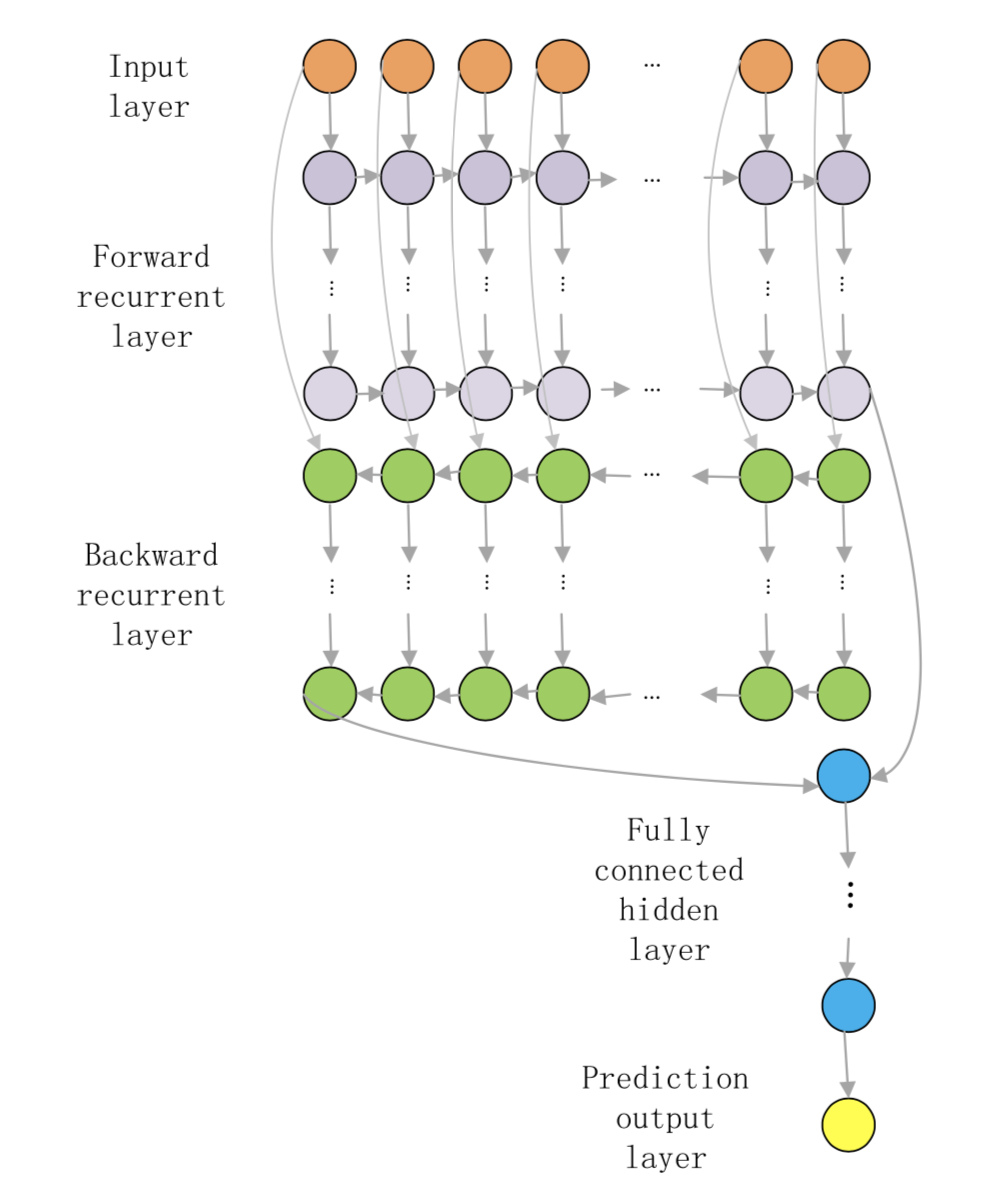
\includegraphics[width=0.7\textwidth]{fig3.png}
		\caption{NN Architecture from Li et al's work}%\label{book}
		\vspace{-1em}
\end{figure}

After the model was trained, the integrated the neural network to a OpenFlow based SDN and tested it with real-time DDoS attacks. In the training process the achieved an accuracy of 98$\%$ and in the test phase their model can effectively clean the network traffic from DDoS attacks.

Also. Yuan et al. applied RNNs to DDoS attack detection and reduced the error from 7.517$\%$ to 2.103$\%$ compared to conventional methods \cite{yuan_deepdefense:_2017}.

However, the data for DDoS attacks may not be as balanced as the data people used for lab researches. The number of "bad" packets is probably a lot smaller than the normal packets, maybe there is no DDoS attack packets for model training at all. In such cases, anomaly detection algorithms usually perform better than common classification algorithms. Sadly, common anomaly detection algorithms based on statistical learning methods do not easily converge on large datasets. Luckily, Chalapathy et al came up with a one-class neural network \cite{chalapathy_anomaly_2018}, which combined deep neural networks for latent representation extraction from the data and a SVM like loss function. Their model performs well on sequential data. Hopefully this will be apply to DDoS detection in future researches.

\section{Another Side of the Coin: Threats from GAN and DRL} 

While we are enjoying the convenience brought to DDoS defense by deep learning, we cannot neglect the potential threats posed by it, especially GAN (Generative Adversarial Nets) and DRL (Deep Reinforcement Learning).

GAN, which was proposed by Goodfellow et al, as well as its variations, is often used to generate data which follows a possibility distribution that extremely resembles the distribution followed by training data\cite{NIPS2014_5423}. This technology has already been used to generate fake pictures which look a lot like real ones. Although can be used to generate DDoS attack data in the training process for a DDoS detection model when lacking abnormal packets, GAN can also be used by perpetrators to generate DDoS attack traffic which shares great similarities with legitimate network traffic, making it much more harder to detect and defense such attacks.

DRL, which was proposed by Google DeepMind based on traditional Q-learning algorithms \cite{mnih2015humanlevel} for decision making and gaming, demonstrated its power when a go program built on it defeated the best human go player Lee Sedol \cite{Silver_2016} and later defeated all human on nearly all board games \cite{alphagozero} without prior knowledge from human being. Based on this, we can assume that people can train a deep reinforcement neural network, which uses a deep neural network as the action-value function, and interact with an environment consisting of nowadays DDoS detection and defense algorithms. By using how many attack packets bypass the defense system as the reward function in this DRL system, given enough training time, we may get a DDoS attack system that can bypass nearly all the defense systems, which will be a great threat to our network infrastructures.

\section{Conclusion and Future Work}

Compared to conventional machine learning algorithms, deep learning shows great potential in the detection and defense against modern DDoS attacks. However, the potential threats brought by deep learning can also not be neglected. 

Future work should concentrate on two aspects: one is to apply deep learning anomaly detection method to network abnormalities detection, and the other is to investigate how GAN and DRL will shape the form of future DDoS attacks.









\newpage
        \bibliographystyle{apacite}
        \bibliography{myref.bib}
\end{document}



%\begin{align} 
%\begin{split}
%(x+y)^3 	&= (x+y)^2(x+y)\\
%&=(x^2+2xy+y^2)(x+y)\\
%&=(x^3+2x^2y+xy^2) + (x^2y+2xy^2+y^3)\\
%&=x^3+3x^2y+3xy^2+y^3
%\end{split}					
%\end{align}

%\begin{table}[htbp]
 %   \centering
  %  \caption{Expected delay and outgoing line of C}
   % \begin{tabular}{ccc}
   % \hline
   % To &Delay & Line \\
   % \hline
   % A&10&B\\
   % B&5&B\\
   % C&0&-\\
   % D&4&D\\
   % E&3&E\\
   % F&8&D\\
   % \hline
   % \end{tabular}
%\end{table}



%\begin{tabbing}
%\hspace*{.25in} \= \hspace*{.25in} \= \hspace*{.25in} \= \hspace*{.25in} \= \hspace*{.25in} \=\kill
%\>$Euclid(m,n)=$ \\
%\>\> {\bf while} n$ \neq $ 0 \\
%\>\>\> r $ \leftarrow $ $m$ mod $n$  \\
%\>\>\>  m $\leftarrow$n\\
%\>\>{\bf return} m 
%\end{tabbing}

%Python code:
%\begin{lstlisting}[language = python]
%def gcd(m,n):
%	while n != 0:
%		r = m % n
%		m = n
%		n = r
%	return m
%\end{lstlisting}


%\paragraph{Heading on level 4 (paragraph)}




%\begin{tabbing}
%	\hspace*{.25in} \= \hspace*{.25in} \= \hspace*{.25in} \= \hspace*{.25in} \= \hspace*{.25in} \=\kill
%	{\bf function} find (A,x,n)\\
%	\> j $\leftarrow$ 0\\
%	\> {\bf while} j < n\\
%	\>\> {\bf if} A[j]=x\\
%	\>\>\>  {\bf return} j  \\
%	\>\> j $\leftarrow$ j+1\\
%	\> {\bf return} -1
%\end{tabbing}


%\begin{figure}[htbp!]
%		\centering
%		\includegraphics[width=0.6\textwidth]{lec26.png}
%		\caption{Linked List}%\label{book}
%		\vspace{-1em}
%\end{figure}


%\begin{wrapfigure}{l}{0.4\textwidth} % Inline image example
 %               \begin{center}
  %              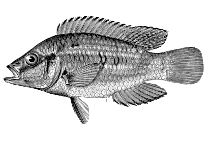
\includegraphics[width=0.38\textwidth]{fish.png}
   %             \end{center}
    %            \caption{Fish}
     %   \end{wrapfigure}



%\begin{align}
%A = 
%\begin{bmatrix}
%A_{11} & A_{21} \\
%A_{21} & A_{22}
%\end{bmatrix}
%\end{align}






